\documentclass{article}
\usepackage[utf8]{inputenc}
\usepackage{graphicx}
\graphicspath{ {images/} }

\title{BDSA Assignment 0}
\author{Jakob Lyngsie Hjalgrim (jlhj@itu.dk)}
\date{10/09-2021}

\begin{document}

\maketitle

\section{Visualization of leap year algorithm}
\begin{center}
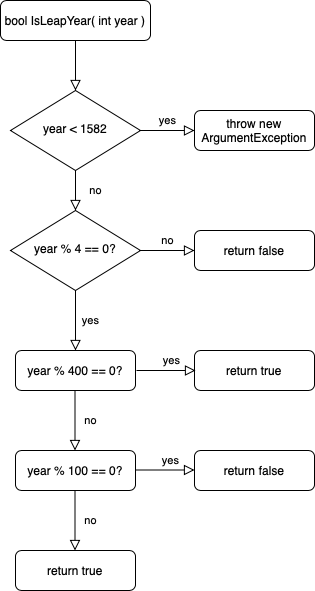
\includegraphics[width=0.4\textwidth]{leapyear_flowchart.png}
\end{center}
The IsLeapYear algorithm determines whether a given year, represented by an integer,
is a leapyear or not. \\
First and foremost the given year must be above 1582 otherwise the IsLeapYear function will throw an ArgumentException, kill the program and present a message saying: "The year must be 1582 or above". If the given year is 1582 or above, the algorithm will further determine certain conditions. \\
If the year is not divisible by 4 the function will return false and write in the Console "nay". If the year is divisible by 4, it will then ask if the year is divisible by 400. If true the function will return true and write in the console "yay".\\
If the year is not divisible by 400, the function will check if the year is divisible by 100. If so it will return false and write in the console "nay". If it is not divisible by 100 the year is divisible by 4 and it will return true, while "yay" will be written in the Console.
\end{document}